\documentclass[12pt]{article}
\usepackage[utf8]{inputenc}
\usepackage{graphicx} % Allows you to insert figures
\usepackage{subcaption}
\usepackage{amsmath} % Allows you to do equations
\usepackage{fancyhdr} % Formats the header
\usepackage{geometry} % Formats the paper size, orientation, and margins
\usepackage{dirtytalk} % typesetting different types of quotation
\usepackage[english]{babel}
\usepackage{csquotes}
\usepackage{hyperref}
\usepackage{listings}
\usepackage{xcolor}
\usepackage{array}
\usepackage{caption}
\usepackage{graphicx}  % in preamble
\usepackage{float}     % in preamble, for [H] placement

% % Define code style
% \lstset{
%   basicstyle=\ttfamily\small,
%   backgroundcolor=\color{gray!10},
%   frame=single,
%   breaklines=true,
%   postbreak=\mbox{\textcolor{red}{$\hookrightarrow$}\space},
%   keywordstyle=\color{blue},
%   commentstyle=\color{green!50!black},
%   stringstyle=\color{orange},
% }

% Code styling
\lstset{
    basicstyle=\ttfamily\footnotesize,
    backgroundcolor=\color{lightgray!20},
    keywordstyle=\color{blue},
    commentstyle=\color{green!50!black},
    stringstyle=\color{red},
    numbers=left,
    numberstyle=\tiny\color{gray},
    stepnumber=1,
    numbersep=10pt,
    showspaces=false,
    showstringspaces=false,
    showtabs=false,
    frame=single,
    tabsize=2,
    breaklines=true,
    breakatwhitespace=false,
    escapeinside={\%*}{*)},
    morekeywords={void, size, setup, draw, pushMatrix, popMatrix}
}

\linespread{1.25} % About 1.5 spacing in Word
\setlength{\parindent}{0.8cm} % No paragraph indents
\setlength{\parskip}{0em} % Paragraphs separated by one line
\renewcommand{\headrulewidth}{0pt} % Removes line in header
\geometry{a4paper, portrait, margin=1in}
\setlength{\headheight}{14.49998pt}
\graphicspath{ {images/} }

\begin{document}
\begin{titlepage}
   \begin{center}
    \textsc{\large Ministry of Education of Republic of Moldova}\\[0.5cm]
    \textsc{\large Technical University of Moldova}\\[0.5cm]
    \textsc{\large Faculty of Computers, Informatics and Microelectronics}\\[0.5cm]
    \textsc{\large Department of Physics}\\[1.2cm]
    
    \vspace{25 mm}
    
    \textsc{\Large Criptography and security}\\[0.5cm]
    \textsc{\large Laboratory work \#4}\\[0.5cm]    % <<<<<<< CHANGE LAB NUMBER HERE
    
    \newcommand{\HRule}{\rule{\linewidth}{0.5mm}}
    \vspace{10 mm}
    \HRule \\[0.4cm]
    { \LARGE \bfseries Block ciphers. DES algorithm}\\[0.4cm] % <<<<<<< CHANGE LAB TITLE HERE
    \HRule \\[1.5cm]
    
    \vspace{10mm}
    
    \begin{minipage}[t]{0.4\textwidth}
    \begin{flushleft} \large
    \emph{Author:} \\
    Dmitrii \textsc{Belih}\\                         % <<<<<<< CHANGE YOUR NAME HERE
    std. gr. FAF-232                                % <<<<<<< CHANGE GROUP NUMBER HERE
    \end{flushleft}
    \end{minipage}
    ~
    \begin{minipage}[t]{0.4\textwidth}
    \begin{flushright} \large
    \emph{Verified:} \\
    \textsc{Zaica} M.\\
    \end{flushright}
    \end{minipage}\\[3cm]
    
    \vspace{5 mm}
    \large Chișinău 2025\\[0.5cm]
    
    \vfill
    \end{center}
\end{titlepage}

\setcounter{page}{2}
\pagestyle{fancy}
\fancyhf{}
\rhead{\thepage}
\lhead{FAF-232 Belih Dmitrii; Laboratory Work №4}




% \section*{Introduction}
\section*{Theory Background}
\hspace{0.8cm}

The Data Encryption Standard (DES) is a symmetric key block cipher developed by IBM in the early 1970s and adopted by the U.S. National Bureau of Standards (NBS) in 1977 as a federal standard (FIPS PUB 46). DES encrypts data in 64-bit blocks using a 56-bit key. Its design is based on the Feistel cipher structure, which divides the data block into two halves and processes them through multiple rounds of substitution and permutation.

\subsection*{Structure of DES}
DES uses a 16-round Feistel network, meaning that the encryption process consists of 16 similar stages or rounds. Each round uses a subkey derived from the main key. The overall structure can be summarized as follows:

\begin{enumerate}
    \item Initial Permutation (IP)
    \item Sixteen Feistel rounds
    \item Final Permutation (IP$^{-1}$)
\end{enumerate}

The Feistel structure allows the same algorithm to be used for both encryption and decryption, differing only in the order of the subkeys.

\subsection*{Initial Permutation (IP)}
Before the 16 rounds begin, DES applies an \textit{initial permutation} (IP) to the 64-bit plaintext. This permutation rearranges the bits of the plaintext according to a predefined table. Although IP does not contribute to the security of DES, it was included for hardware efficiency in the original design.

\subsection*{The Feistel Function}
Each round of DES uses a function \( f(R_{i-1}, K_i) \), where \( R_{i-1} \) is the right half of the data and \( K_i \) is the round subkey. The function consists of the following steps:

\begin{enumerate}
    \item \textbf{Expansion (E-box):} The 32-bit \( R_{i-1} \) is expanded to 48 bits.
    \item \textbf{Key Mixing:} The expanded block is XORed with the 48-bit round key \( K_i \).
    \item \textbf{Substitution (S-boxes):} The result is divided into eight 6-bit blocks, each substituted by a 4-bit output using one of eight substitution boxes (S-boxes).
    \item \textbf{Permutation (P-box):} The 32-bit output from the S-boxes is permuted using a fixed P-box.
\end{enumerate}

Finally, the result of \( f(R_{i-1}, K_i) \) is XORed with the left half \( L_{i-1} \) of the previous round to produce the new right half:
\[
L_i = R_{i-1}, \quad R_i = L_{i-1} \oplus f(R_{i-1}, K_i)
\]

\subsection*{Key Generation Process}
The key schedule in DES generates sixteen 48-bit round keys from the original 56-bit key. The process is as follows:

\begin{enumerate}
    \item Apply the \textit{Permuted Choice 1 (PC-1)} to select 56 bits from the 64-bit key (8 bits are used for parity).
    \item Split the key into two 28-bit halves (\( C_0 \) and \( D_0 \)).
    \item For each round \( i \), the halves are shifted left by 1 or 2 bits according to a predefined schedule.
    \item Apply the \textit{Permuted Choice 2 (PC-2)} to produce the 48-bit round key \( K_i \).
\end{enumerate}

\subsection*{Encryption and Decryption}
The encryption process consists of applying the 16 Feistel rounds to the permuted plaintext. The final result is the ciphertext obtained after applying the inverse initial permutation (IP$^{-1}$).

Decryption in DES uses the same process but with the subkeys applied in reverse order (\( K_{16}, K_{15}, \ldots, K_1 \)) due to the symmetric nature of the Feistel structure.

\section*{The Task}

Develop a program in one of the student's preferred programming languages to implement an element of the DES (Data Encryption Standard) algorithm.  
The specific task assigned to each student is determined by their position number \(n\) in the group list, using a given formula ex = n mod 11, where \(n\) corresponds to the list of students number.


\textbf{My Variant:} \\
Given K+ in the DES algorithm, determine Ci and Di for a given i.

\section*{Technical implementation}
\hspace{0.8cm}
In DES, the 56-bit key \( K^{+} \) is split into two halves:
\[
C_0 = K^{+}[1..28], \quad D_0 = K^{+}[29..56]
\]
At each round \( i \), both halves are cyclically shifted to the left by either one or two positions, depending on the round number.  
The number of left shifts for each iteration is defined in the DES shift schedule:

    \begin{lstlisting}[language=Java]
        iteration = {
    1: 1, 2: 1, 3: 2, 4: 2, 5: 2, 6: 2, 7: 2, 8: 2,
    9: 1, 10: 2, 11: 2, 12: 2, 13: 2, 14: 2, 15: 2, 16: 1
}
    \end{lstlisting}

\subsection*{Program Description}

The program is implemented in Python and performs the following steps:

\begin{enumerate}
    \item \textbf{Define the iteration table:}  
    A dictionary named \texttt{iteration} is used to represent the shift schedule for each round \( i \).


\begin{verbatim}
    
iteration = {
    1: 1, 2: 1, 3: 2, 4: 2, 5: 2, 6: 2, 7: 2, 8: 2,
    9: 1, 10: 2, 11: 2, 12: 2, 13: 2, 14: 2, 15: 2, 16: 1
}
\end{verbatim}

    \item \textbf{Generate or input a 56-bit key:}  
    The user can either enter their own \( K^{+} \) value or use a randomly generated 56-bit binary string.
\begin{verbatim}
k_random = ""
while len(k_random) < 56:
    k_random += str(random.randint(0, 1))
\end{verbatim}

    \item \textbf{Validate key length:}  
    The program checks that \( K^{+} \) is exactly 56 bits long.

    \item \textbf{Split into two halves:}  
    The 56-bit key is divided into two 28-bit halves:
\begin{verbatim}
c0 = kplus[:28]
d0 = kplus[28:]
\end{verbatim}

    \item \textbf{Read the round number \( i \):}  
    The user inputs a round number \( i \), and the program verifies that \( i \in [1,16] \).

    \item \textbf{Calculate total shift:}  
    The total number of shifts up to iteration \( i \) is computed by summing the shift values from the iteration table.
\begin{verbatim}
count = 0
for j in iteration.keys():
    if j <= i_value:
        count += iteration[j]
\end{verbatim}

    \item \textbf{Perform circular shifts:}  
    The left and right halves \( C_0 \) and \( D_0 \) are circularly shifted left by the total number of positions (\texttt{count}) to obtain \( C_i \) and \( D_i \).
\begin{verbatim}
c_new = c0[count:] + c0[:count]
d_new = d0[count:] + d0[:count]
\end{verbatim}

    \item \textbf{Display results:}  
    The program prints:
    \begin{itemize}
        \item The iteration table
        \item The initial halves \( C_0 \) and \( D_0 \)
        \item The total shift value
        \item The computed \( C_i \) and \( D_i \)
        \item All intermediate values for verification
    \end{itemize}
\end{enumerate}

Full code of the program:
    \begin{lstlisting}[language=Java]
import random

iteration = {
    1: 1,
    2: 1,
    3: 2,
    4: 2,
    5: 2,
    6: 2,
    7: 2,
    8: 2,
    9: 1,
    10: 2,
    11: 2,
    12: 2,
    13: 2,
    14: 2,
    15: 2,
    16: 1,
}

print(iteration.keys())
print(iteration[16])

k_random = ""

while len(k_random) < 56:
    k_random += str(random.randint(0, 1))

print(len(k_random))
print(k_random)

kplus = input("Enter kplus value: ")
if len(kplus) == 56:

    print(iteration)
    print(kplus)

    c0 = ""
    d0 = ""
    for i in range(len(kplus) // 2):
        c0 += str(kplus[i])

    for i in range(len(kplus) // 2):
        d0 += str(kplus[i + len(kplus) // 2])

    print(c0)
    print(d0)

    i_value = int(input("Write i value: "))
    if i_value < 17 and i_value > 1:
        print("i value is correct")
        count = 0
        for i in iteration.keys():
            if i <= i_value:
                count += iteration.get(i)
                print(iteration.get(i))
            else:
                break

        print("-------------------------------")
        print(iteration.get(i_value))

        print("-------------------------------")
        print(count)

        c_new = c0[count:] + c0[:count]
        d_new = d0[count:] + d0[:count]

        print(c_new + " C of iteration: " + str(i_value))
        print(d_new + " D of iteration: " + str(i_value))

        for i in range(i_value + 1):
            c_all = c0[i:] + c0[:i]
            d_all = d0[i:] + d0[:i]
            print("-------------------------------")
            print(c_all + " C iteration: of " + str(i))
            print(d_all + " D iteration: of " + str(i))
    else:
        print("i value must be between 1 and 16")

else:
    print("kplus must be 56 characters long")

    \end{lstlisting}

\section*{Results}
\hspace{0.8cm}

\begin{figure}[H]
    \centering
    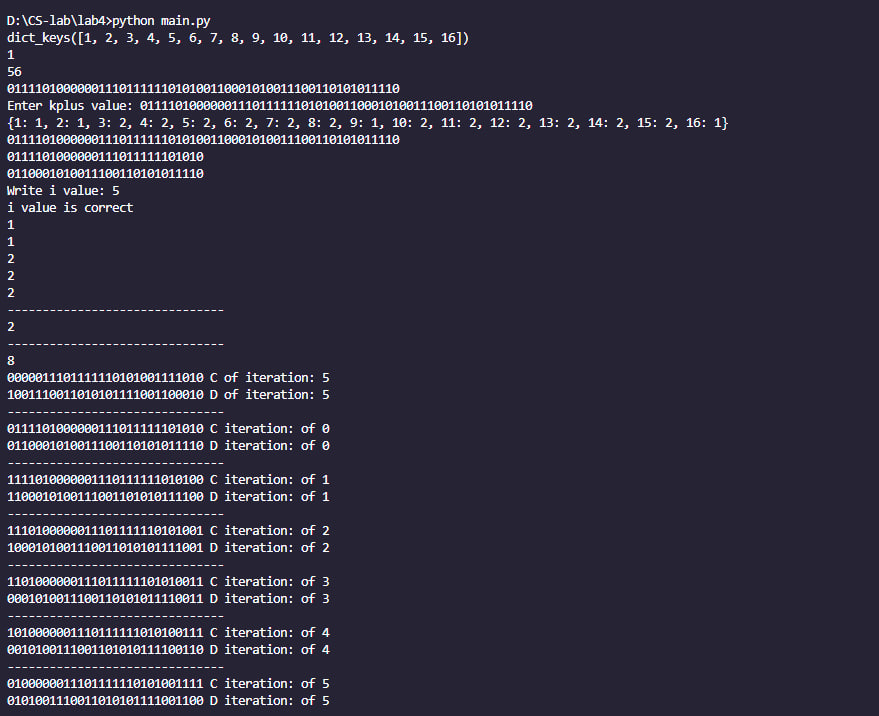
\includegraphics[width=0.8\textwidth]{img/das.jpg}  % Use relative width
    \caption{Program execution showing the system}
    \label{fig:example}
\end{figure}

% \textit{Task1}

% \begin{figure}[h!]
%     \centering
%     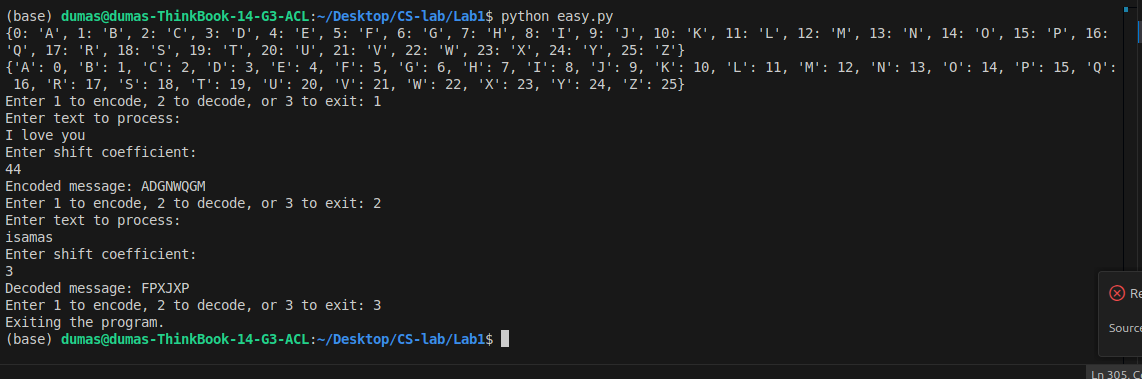
\includegraphics[width=0.8\textwidth]{img/Res1.png}
%     \caption{Result of the encoding and decoding program}
%     \label{fig:result1}
% \end{figure}

% \textit{Task2}

% \begin{figure}[h!]
%     \centering
%     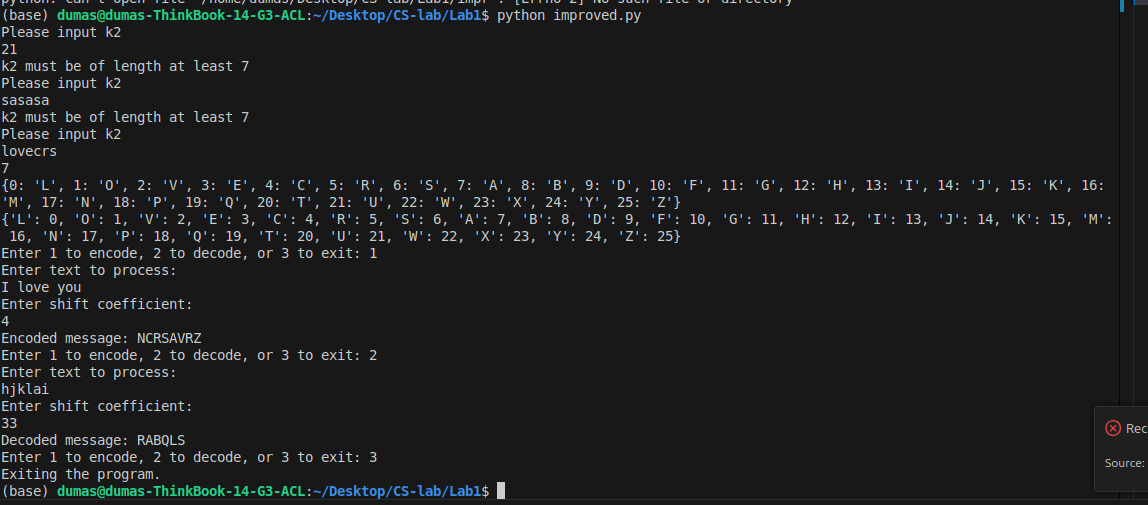
\includegraphics[width=0.8\textwidth]{img/Res2.png}
%     \caption{Result of the encoding and decoding program}
%     \label{fig:result1}
% \end{figure}





\section*{Conclusion}
\hspace{0.8cm}

In this lab, we implemented a key step of the Data Encryption Standard (DES) algorithm: generating the intermediate keys \(C_i\) and \(D_i\) from the 56-bit key \(K^{+}\). The program allows both manual and random input of the key and calculates the left and right halves for a given iteration \(i\) according to the DES shift schedule.

Through this exercise, we gained practical experience in understanding the DES key schedule and the role of cyclic shifts in subkey generation, splitting the 56-bit key into halves and applying iterative left rotations, displaying intermediate steps to verify the correctness of the algorithm, and writing a program that combines theoretical knowledge with computational implementation.

Overall, this lab helped us understand the inner workings of DES key management and reinforced the importance of careful handling of keys and iterative transformations in symmetric cryptography. The results demonstrate that the algorithm produces correct \(C_i\) and \(D_i\) values, providing a solid foundation for implementing full DES encryption and decryption in future tasks.





\pagebreak
\end{document}